	\documentclass[../pfc.tex]{subfiles}
		
	\begin{document}
	
Para la fase de análisis dentro de las metodologías ágiles no existen preceptos firmes a cumplir, pero dado que se valora mucho la comunicación y las relaciones interpersonales, se establece que debería haber una serie de reuniones previas al inicio de los sprints para que el equipo pueda obtener contexto del proyecto y del dominio del mismo, así como ir escribiendo las historias de usuario y rellenar y priorizar el product backlog. En estas reuniones idealmente asistirían tanto el product owner, el scrum master y el equipo, pero con el product owner, el scrum master y aquel del equipo que mejor pueda ayudar a escribir las historias puede ser suficiente, recordemos que no se está estimando, simplemente se escuchan las necesidades del product owner y estas se traducen en funcionalidades y estas a su vez en requisitos mediante historias de usuario.\\*

Para acometer el trabajo y dividirlo en trozos mas manejables en estos casos se suele recurrir a escribir historias épicas, que más tarde ya si pueden particionar el scrum master y el equipo para posteriormente remitirlas al product owner para que este exprese su conformidad o sus matices a las historias de usuario ya redactadas en piezas manejables y que priorice el product backlog inicial, teniendo en cuenta que tras la estimación inicial puede haber algún reordenamiento para aprovechar mejor los tiempos del sprint.\\* 

Una vez las historias tienen una forma más o menos fija, recordemos que uno de los fines del agilismo es responder al cambio y más aún al cambio en los requisitos, se hace una reunión de estimación de las mismas. Como ya se ha comentado existen varias maneras de estimar la complejidad que suponen las historias de usuario, casi todas basadas en variaciones del poker planning que se explicó anteriormente.\\* 

En el momento de redactar las historias de usuario conviene que de algún modo alguien, típicamente el scrum master o el product owner, se encargue de recordar los grandes objetivos del proyecto. Estos objetivos son los objetivos claros, concisos y lo mas sencillos posibles que mueven al cliente a dar comienzo al proyecto. Todas las historias de usuario, así como las acciones que se lleven a cabo, deben alinearse con estos objetivos.\\*


Para llevar a cabo todo este proceso se llevaron a cabo varias reuniones con el personal de la AECC, se cruzaron correos con historias redactadas, se conversó vía Hangout, Skype, Whatsapp, etc se volvió a reunir las veces que hicieron falta, hasta que dicho personal, que en este caso hacía el papel de product owner,  se sintió lo suficientemente cómodo con el redactado inicial de las historias de usuario y su priorización, sabiendo que después estas podrían modificarse.\\*
	

	\section{Explicación detallada de las funcionalidades de la aplicación}

Este sería el proceso donde algún miembro del equipo ganaría contexto por parte del product owner, al este describirle lo que quiere, vamos a pasar al redactado final de las necesidades que se expresaron, pues debido a la inexperiencia de los miembros de la AECC en el mundo de la movilidad el punto de partida del proyecto estaba mucho más alejado de aquí. Esto en el argot del agilismo se llama educar al cliente, y como siempre se basa en la comunicación, las relaciones interpersonales y en la confianza mutua.\\*

\textbf{USO SIN REGISTRO}

En todo momento se debe poder usar la app sin hacer ningún tipo de registro previo. Solamente algunas funcionalidades especificas necesitarán del mismo. Para ello los datos serán almacenados en el dispositivo, sin perjuicio de que puedan una vez registrado ser compartidos en 'la nube' y se carguen en varios dispositivos.\\*

	\textbf{PRINCIPAL}
	
	Este será el punto de entrada habitual a la aplicación. salvo la primera vez que se ofrecerá la posibilidad de realizar un pequeño tutorial en la misma. Al entrar en la misma se obtiene un pequeño resumen con los eventos de todo tipo próximos en el día de hoy o un texto que nos informe de la ausencia de algún tipo de evento para el día de hoy.\\*

	
	\textbf{PERSONAJES}
	
	Una pequeña lista de contactos importantes relacionados con la enfermedad, como puedan ser el oncólogo, el psicólogo, familiares de especial relevancia, etc.
	
	Como toda lista de contactos podrán añadirse, modificarse, borrarse y consultarse cada uno de los ítems que la componen de una manera sencilla, siguiendo los lineamientos del SO en cuestión.\\*
	
	Por cuestiones de practicidad y simplicidad, si se añade un contacto o se modifica en esta parte, lo hará también en la app general de contactos del SO. Esto es así para que en cualquiera de las listas el usuario pueda encontrar al contacto que busque y no se sienta desorientado manejando varias listas de contactos en el dispositivo móvil. \\*
	
	\textbf{CITAS}
	
	Es una funcionalidad para introducir citas médicas en un calendario. En las mismas se podrá añadir al profesional que nos atiende si es que se conoce. 
	Poco después de una cita se generará una notificación preguntando por la misma, en la que se preguntará si la cita ha generado nuevas citas, momento en que se pasará a la pantalla para crear una nueva cita, si ha habido cambios en la medicación, yendo a la lista de medicamentos para añadir o cambiar la dosis de los mismos.
	Poco antes de la cita y siguiendo las pautas marcadas en el folleto se guiará al usuario en las actividades o como afrontar la cita.
	Lista de citas Nombre de la cita, fecha y hora.

	Desde el propio ítem de la lista se podrán añadir medicamentos, personas, síntomas y/o pruebas, al pulsar sobre la opción correspondiente nos llevará al listado de estás opciones añadiéndose así.\\*
	
	\clearpage
	
	\textbf{AVATAR}
	
	En esta funcionalidad se permite crear un perfil de registro al usuario de la app para acceder a alguna funcionalidad mas, como compartir los datos entre dispositivos, mediante el uso de un servicio de back end que almacene los nuevos datos cuando se disponga de conectividad. El acceso a tratar con un agente como parte del piloto del proyecto, pudiéndole dejar alguna pregunta que desde la parte servidora se encargara de responder.\\*

	\textbf{RUTINA}
	
	La rutina es una vista semanal de actividades programadas y de ritmo de vida. Se pueden introducir actividades reiterativas y en que consisten, si se hacen solo o en grupo y la satisfacción que el usuario estima que producen. De vez en cuando aparecerán notificaciones que pregunten si se realizo o no una actividad determinada, si esta causo satisfacción etc. Puede marcarse en este horario la hora en la que el usuario se levanta y acuesta para excluir notificaciones en ese horario de descanso. \\*
	Revisar esta página	https://code.google.com/p/yadview/\\*
		
	
	\textbf{MEDICACIÓN}
	
	Es un gestor de aquellos medicamentos que debe tomar el enfermo y en que cantidades, así como histórico de las tomas de los mismo o de alguno que no tengan prescrito como pudieran ser analgésicos, antidepresivos, etc 
	
	La app debe avisar con una notificación de la necesidad de toma de aquellos medicamentos que se marquen como prescritos por el facultativo, a partir de la posología indicada para el mismo. \\*

	\textbf{PRUEBAS}
	
	Es una funcionalidad para llevar un registro de las pruebas que se han realizado al paciente clasificadas por tipos y llegado el caso hacer seguimiento de los valores clave en cada prueba diagnostica o análisis Se podrán adjuntar fotografiás de los resultados en papel si es que se dispone de ellos para disponer de un pequeño "registro documental".\\*
	
	\textbf{SÍNTOMAS y ANOTACIONES}
	
	Esta funcionalidad cubre anotaciones de síntomas, sensaciones y cualquier cosa que el paciente crea conveniente anotar. Antes de una cita le recordará que tiene anotaciones por si quisiese comentárselas al profesional y también permitirá pasar una anotación para la siguiente cita.\\*

	\textbf{INFORMACIÓN ÚTIL}
	
	Una sección con los consejos de vida sana, meditación, relajación etc que también disponen en el folleto pero con un enfoque más accesible y con algún tema relajante para facilitar la relajación del usuario.\\* 
	
	\textbf{PARTE SERVIDORA}

	El back end almacenara los datos que los usuarios registrados envíen desde sus dispositivos y los devolverá hacia aquellos que no se encuentren sincronizados. Ademas permitirá a un rol supervisor provincia asociar a un usuario registrado a un agente que desde ese momento velara por el. Dicho agente podrá comunicarse con el usuario de manera directa y también respondiendo a sus preguntas.\\*  

	\clearpage
	
	\section{Documento de Análisis}

	Como se ha comentado anteriormente es difícil capturar todos los requisitos y el contexto de la aplicación a partir de una reunión, en nuestro caso mantuvimos al menos cuatro reuniones presenciales y al menos casi otras tantas por medios telemáticos al residir en provincias diferentes y además contamos con la ayuda del folleto que querían "digitalizar" "Mis Cuidados, diario de salud para supervivientes de cáncer".\\*
			
	Una de las ventajas de utilizar este primer tipo de metodología, es el de poder adaptar de una manera mucho más eficiente los recursos a las fechas y a los requisitos, y poder modificar estos requisitos de manera 'ágil' debido al panorama cambiante que podemos tener de cara al cliente.\\*
			
		
	\subsection{Descripción de objetivos de manera detallada}
	
	
	\textbf{OBJ-001}	La aplicación deberá poder usarse en un dispositivo sin registro y sin conexión.\\*
	
	\textbf{OBJ-002}	La aplicación debe ser fácil de usar para usuarios no avanzados y personas mayores.\\*
	
	\textbf{OBJ-003}	Cualquier opción que se pueda realizar en el folleto debe estar cubierta por alguna funcionalidad de la app.\\*
	
	\textbf{OBJ-004}	Se hará énfasis en que el registro proporciona grandes ventajas, a pesar de poder usarse sin él.\\*

	\textbf{OBJ-005}	El estilo gráfico de la app sera coherente con el marcado por el folleto de la AECC.\\*
	
	\textbf{OBJ-006}	En definitiva la app será algo útil por su funcionalidad pero también por su usabilidad y facilidad de manejo.\\*
	
	
	\subsection{Captura de Requisitos}
	
	Como consecuencia de las diferentes reuniones realizadas con el cliente se elabora un documento de especificación de requisitos con el propósito de describir las funcionalidades necesarias para poder validar el producto final.
	
	Estos requisitos se escriben aquí como historias de usuario con un id, un titulo y una descripción para ser implementadas. \\*
	
	\subsubsection{Historias de usuario}
			
	\textbf{Historia 1: Navegación}

		Como usuario quiero poder acceder al menú de navegación desde cualquier punto del primer nivel de la misma, mediante la pulsación en el icono de tres lineas en la izquierda de la pantalla, para poder navegar entre las distintas opciones de la app. Dejando en el resto de niveles de navegación una flecha para volver al nivel 1.\\*
		
		
	\textbf{Historia 2: Registro}
		
		Como usuario quiero poder registrarme, acceder y modificar mas tarde estos datos para poder acceder a las funcionalidades de sincronización y consulta con agente.\\*
	
	
	\textbf{Historia 3: Personas}
		
		Como usuario quiero poder añadir, consultar, modificar y borrar uno de los contactos de la lista de personas relacionadas desde la app y que estos cambios se reflejen también en la app de contactos para poder tener un listado de personas importantes.\\*


	\textbf{Historia 4: Citas}	
	
		Como usuario quiero poder añadir, consultar modificar y borrar citas medicas con los datos de lugar, fecha, hora, especialista para poder tener un control de mis citas y que estas pasen a la app calendario del dispositivo. \\*
		
		
	\textbf{Historia 5: Notificaciones citas}
		
		Como usuario quiero que la app me avise de las citas próximas en la manera en la que el folleto lo indica para poder preparar la cita de cara a sacarle el máximo partido.\\*
	
	
	\textbf{Historia 6: Principal}
	
		Como usuario al entrar en la aplicación quiero que me muestre el siguiente evento hoy si lo hubiese de cada una de las categorías: citas, medicación, horarios, etc para poder tener una idea aproximada del día.\\*
	
	
	\textbf{Historia 7: Rutina}
	
		Como usuario quiero poder añadir, consultar, modificar y borrar elementos en el calendario semanal de rutinas para poder planificar mis actividades semanales.\\*
	
	
	\textbf{Historia 8: Notificaciones Rutinas}
	
		Como usuario quiero que me la app me avise del comienzo de alguna actividad del horario semanal, así como que me pregunte por algunas de ellas para recabar información de mi estado de ánimo y como me favorece la rutina. \\*
	
	
	\textbf{Historia 9: Medicación}
	
		Como usuario quiero poder introducir, modificar, consultar y borrar información sobre medicamentos que el profesional me prescriba, así como de otros tomados de forma puntual pero de los que tengo registro de que son para poder llevar un histórico de lo que he tomado o poder comentárselo al profesional en las siguientes citas médicas.\\*
	
	
	\textbf{Historia 10: Notificaciones Medicación}
	
		Como usuario quiero que la aplicación me notifique de que debo tomar una determinada medicación para no saltarme ninguna de las prescripciones del profesional. Además si tomo alguna medicación no prescrita quiero que me avise de la misma poco antes de la próxima cita en el tiempo y que me permita pasarla de cita.\\*
	
	
	\textbf{Historia 11: Pruebas}
	
		Como usuario quiero que la aplicación me permita añadir, modificar, consultar y borrar la información referente a una prueba diagnostica o de análisis para poder disponer de un histórico de los valores a tener en cuenta. \\*
	
	
	\textbf{Historia 12: Síntomas y anotaciones}
	
		Como usuario quiero que la aplicación me permita añadir, modificar, consultar y borrar anotaciones libres para consultar en las citas con el profesional para poder comentar con el mismo la gravedad o no de los mismos.\\*
	

	\textbf{Historia 13: Notificaciones Síntomas}
	
		Como usuario de la aplicación quiero que me notifique poco antes de una cita que existen síntomas o comentarios que pueden tener que comentarse con el profesional o poder moverlos a la siguiente cita con otro profesional para poder poner en común con el mismo toda la información que pudiera ser relevante.\\*
	
	
	\textbf{Historia 14: Información Útil}
	
		Como usuario quiero poder consultar toda la información recopilada en el folleto de la AECC para que esta se pueda consultar de una manera sencilla y aprovechar el conocimiento de la misma.\\*
	
	
	\textbf{Historia 15: Servicios Web}
	
		Como usuario registrado quiero disponer de unos servicios web para sincronizar la información entre varios dispositivos.\\*
	
	
	\textbf{Historia 16: Estadísticas}
	
		Como personal de la AECC quiero obtener estadísticas eliminando los datos personales y de identificación para mejorar el conocimiento de la enfermedad y su relación con las actividades que esta aplicación almacena.\\*
	
	
	\textbf{Historia 17: Asignar Usuario}
	
		Como superusuario de la parte servidora quiero poder asignar un usuario registrado de una provincia a uno de los agentes disponibles en la misma para que este sea su agente de referencia.\\*


	\textbf{Historia 18: Vision Agente}
	
		Como agente de la AECC en la parte servidora quiero poder consultar mis supervivientes, consultar sus eventos adversos así como lanzares comunicaciones y que estas les lleguen por notificación push a sus dispositivos\\*
		

	\subsection{Identificación de actores}
	
	Cualquier aplicación necesita interactuar con algún actor, ya sea humano o de software.
	
	Los actores humanos se van a identificar en nuestra aplicación como los distintos tipos de usuario y el propio agente de la AECC que se encarga de la parte servidora y que será el que se encargue de recibir parte de la información que transmita el tipo de usuario y realizar con ella las acciones oportunas.\\*
	
	A continuación se pasará a describir cada uno de los actores identificados en nuestra aplicación:\\*
	
	\textbf{USUARIO NO REGISTRADO}
	Este actor representa a los usuarios que todavía no se han registrado en la aplicación o aquellos que no quieren registrarse e interactúan con la misma. Incluimos también a los usuarios que acceden pon primera vez y no han completado el registro.\\*
	
	\textbf{USUARIO REGISTRADO}
	Este actor representa una generalización de todos los usuarios que pueden interactuar con la aplicación, representa a los usuarios que pueden identificarse en la aplicación después de haberse registrado en la misma.
	
	Los usuarios registrados van a tener una serie de ventajas sobre los que no lo están con forma de atención personalizada por parte de un agente de la AECC que hará de ''ángel de la guarda'' y vigilará de manera sistemática el estado de este usuario.\\*
	
	\textbf{AGENTE DE LA AECC}
	Este actor representa a los agentes de la AECC destinados a hacer un seguimiento de los usuarios registrados en la aplicación, tendrá acceso a la información facilitada por estos últimos y podrá dar una atención personalizada a aquellos a los que tutele.\\*
		
	\subsection{Casos de uso }
		
	Un caso de uso es una descripción de los pasos o las actividades que deberán realizarse para llevar a cabo algún proceso.\\*
	
	Los personajes o entidades que participarán en un caso de uso se denominan actores. En el contexto de ingeniería del software, un caso de uso es una secuencia de interacciones que se desarrollarán entre un sistema y sus actores en respuesta a un evento que inicia un actor principal sobre el propio sistema. Los diagramas de casos de uso sirven para especificar la comunicación y el comportamiento de un sistema mediante su interacción con los usuarios y/u otros sistemas. O lo que es igual, un diagrama que muestra la relación entre los actores y los casos de uso en un sistema. Una relación es una conexión entre los elementos del modelo, por ejemplo la especialización y la generalización son relaciones. Los diagramas de casos de uso se utilizan para ilustrar los requerimientos del sistema al mostrar cómo reacciona a eventos que se producen en su ámbito o en él mismo.\\*
	
	Los más comunes para la captura de requisitos funcionales, especialmente con el desarrollo del paradigma de la programación orientada a objetos, donde se originaron, si bien puede utilizarse con resultados igualmente satisfactorios con otros paradigmas de programación.\\*
	
	Pudiera parecer que las metodologías ágiles no valoran los casos de uso, nada más lejos de la realidad, los casos de uso son el guión de lo que una o varias funcionalidades deben realizar. Es por tanto el nexo de unión entre varias historias, es el guión de test automáticos de validación, es quien atesora las reglas de negocio que deben gobernar en nuestra implementación, y es quien conoce las operaciones y entidades que son necesarias en la aplicación. Por eso para los procesos de pruebas, documentación, elaboración de historias, e implementación son una pieza básica que no debemos perder de vista. Tanto es así que es la piedra sobre la que se erige la aplicación para lograr una arquitectura desacoplada y de calidad. 
	
	WIKIPEDIA
	
	Dado el número de casos de uso existente y que estos quedan descritos por el siguiente apartado, ponemos un ejemplo de uno de ellos, referente a la parte de la medicación.
	
	\begin{figure}[H]
		\centering
		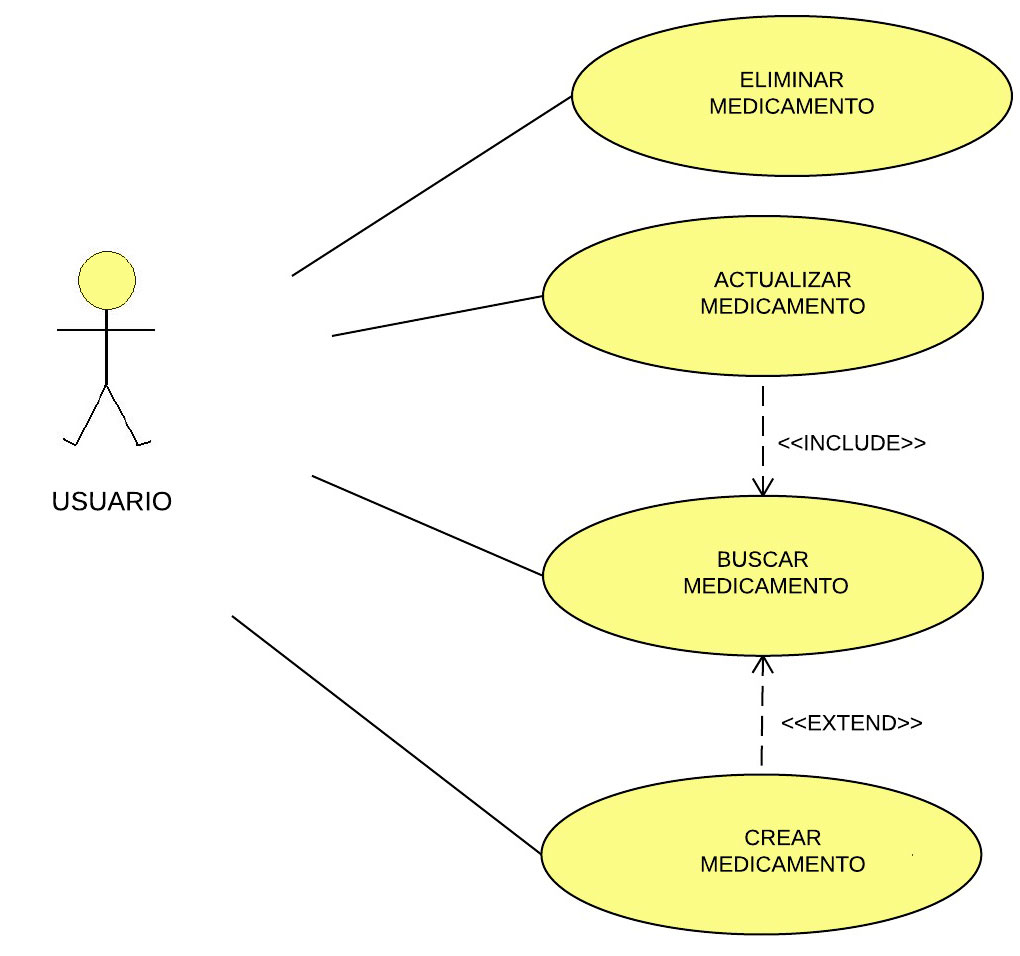
\includegraphics[width=0.7\linewidth]{../images/casodeuso}
		\caption{CRUD de medicamento (caso de uso)}
		\label{fig:casodeusocrud}
	\end{figure}
	
	 
	
	\clearpage

	\subsection{Descripción de Casos de Uso}
	
	\textbf{CASOS DE USO}\\*
	
	\textbf{CU-001} PERFIL DE USUARIO - Inserción\\*
	
	\begin{table}[H]
		\centering
		\begin{tabular}[t]{|p{3cm}|p{9.5cm}|}
				\hline \textbf{CU-001} & \textbf{PERFIL DE USUARIO- INSERCIÓN} \\*
				\hline\hline \textbf{Versión} & 1.0 \\*
				\hline\hline \textbf{Fecha} & 23/07/2015 \\*
				\hline\textbf{Actores} 	& Usuario\\*
				\hline \textbf{Objetivo} & Incluir en la aplicación los datos personales del usuario\\* 			
				\hline \textbf{Precondición} & Los datos del usuario están sin completar \\* 
				\hline \textbf{Flujo normal} & 1.- Desplegamos el menú drawer \\* 
											 & 2.- Pulsamos el círculo que está al principio del menú drawer \\*	
											 & 3.- Completamos los datos personales del usuario\\*	
				\hline \textbf{Flujo alternativo} & 1.- Desplegamos el menú drawer \\* 
 												  & 2.- Pulsamos la opción AJUSTES \\*	
												  & 3.- Pulsamos la opción en pantalla 'Perfil' \\*	
												  & 3.- Completamos los datos personales del usuario \\*	
				\hline \textbf{Postcondición} & El usuario posee sus datos personales en la aplicación \\* 
				\hline \textbf{Comentarios}   & A la hora de introducir la fotografía dentro de los datos personales, podrá elegir entre las que tenga en la galería del propio terminal o acceder a la aplicación de cámara para hacer una nueva fotografía\\*
				\hline
			\end{tabular}
			\caption{Perfil de usuario - Inserción}
			\label{tabla:caso001}
	\end{table}
		
	\textbf{CU-002}	PERFIL DE USUARIO - Consulta\\*
	
	\begin{table}[H]
		\centering
		\begin{tabular}[t]{|p{3cm}|p{9.5cm}|}
			\hline \textbf{CU-002} & \textbf{PERFIL DE USUARIO - CONSULTA} \\*
			\hline\hline \textbf{Versión} & 1.0 \\*
			\hline\hline \textbf{Fecha} & 24/07/2015 \\*
			\hline\textbf{Actores} 	& Usuario\\*
			\hline \textbf{Objetivo} & Consultar en la aplicación los datos personales del usuario\\* 			
			\hline \textbf{Precondición} & Los datos del usuario existen en la aplicación \\* 
			\hline \textbf{Flujo normal} & 1.- Desplegamos el menú drawer\\* 
			& 2.- Pulsamos el círculo que está al principio del menú drawer\\*	
			& 3.- Consultamos los datos personales del usuario\\*	
			\hline \textbf{Flujo alternativo} & 1.- Desplegamos el menú drawer\\* 
			& 2.- Pulsamos la opción AJUSTES \\*	
			& 3.- Pulsamos la opción en pantalla 'Perfil' \\*	
			& 3.- Consultamos los datos personales del usuario \\*	
			\hline \textbf{Postcondición} & El usuario ha consultado sus datos personales\\* 
			\hline \textbf{Comentarios}   & Se pueden consultar todos los datos referentes al perfil del usuario\\*
			\hline
		\end{tabular}
		\caption{Perfil de usuario - Consulta}
		\label{tabla:caso002}
	\end{table}
	
	\clearpage
	
	\textbf{CU-003} PERFIL DE USUARIO - Edición\\*
	
	\begin{table}[H]
		\centering
		\begin{tabular}[t]{|p{3cm}|p{9.5cm}|}
			\hline \textbf{CU-003} & \textbf{PERFIL DE USUARIO - EDICIÓN} \\*
			\hline\hline \textbf{Versión} & 1.0 \\*
			\hline\hline \textbf{Fecha} & 24/07/2015 \\*
			\hline\textbf{Actores} 	& Usuario\\*
			\hline \textbf{Objetivo} & Modificar en la aplicación los datos personales del usuario\\* 			
			\hline \textbf{Precondición} & Los datos del usuario existen en la aplicación \\* 
			\hline \textbf{Flujo normal} & 1.- Desplegamos el menú drawer\\* 
			& 2.- Pulsamos el círculo que está al principio del menú drawer\\*	
			& 3.- Completamos los datos personales del usuario que queramos cambiar\\*	
			\hline \textbf{Flujo alternativo} & 1.- Desplegamos el menú drawer\\* 
			& 2.- Pulsamos la opción ajustes \\*	
			& 3.- Pulsamos la opción en pantalla 'Perfil' \\*	
			& 3.- Completamos los datos personales del usuario que queramos cambiar\\*	
			\hline \textbf{Postcondición} & El usuario posee sus datos personales modificados\\* 
			\hline \textbf{Comentarios}   & El usuario puede a su elección dejar los datos tal y como estuviesen en un principio\\*
			\hline
		\end{tabular}
		\caption{Perfil de usuario - Edición}
		\label{tabla:caso003}

	\end{table}
		
	\textbf{CU-004}	PERFIL DE USUARIO - Borrado\\*

	\begin{table}[H]
		\centering
		\begin{tabular}[t]{|p{3cm}|p{9.5cm}|}
			\hline \textbf{CU-004} & \textbf{PERFIL DE USUARIO - BORRADO} \\*
			\hline\hline \textbf{Versión} & 1.0 \\*
			\hline\hline \textbf{Fecha} & 24/07/2015 \\*
			\hline\textbf{Actores} 	& Usuario\\*
			\hline \textbf{Objetivo} & Borrar de la aplicación los datos personales del usuario\\* 			
			\hline \textbf{Precondición} & Los datos del usuario existen en la aplicación \\* 
			\hline \textbf{Flujo normal} & 1.- Desplegamos el menú drawer \\* 
			& 2.- Pulsamos el círculo que está al principio del menú drawer\\*	
			& 3.- Eliminamos los datos personales del usuario\\*	
			\hline \textbf{Flujo alternativo} & 1.- Desplegamos el menú drawer \\* 
			& 2.- Pulsamos la opción ajustes \\*	
			& 3.- Pulsamos la opción en pantalla 'Perfil' \\*	
			& 3.- Eliminamos dos datos del usuario\\*	
			\hline \textbf{Postcondición} & El usuario ha eliminado sus datos personales\\* 
			\hline \textbf{Comentarios}   & El usuario puede a su elección dejar los datos tal y como estuviesen en un principio\\* 
			\hline
		\end{tabular}
		\caption{Perfil de usuario - Borrado}
		\label{tabla:caso004}

	\end{table}
	
	\clearpage
	
	\textbf{CITA MÉDICA}\\*

	\textbf{CU-005}	CITA MÉDICA - Inserción\\*
	
	\begin{table}[H]
		\centering
		\begin{tabular}[t]{|p{3cm}|p{9.5cm}|}
			\hline \textbf{CU-005} & \textbf{CITA MÉDICA - INSERCIÓN} \\*
			\hline\hline \textbf{Versión} & 1.0 \\*
			\hline\hline \textbf{Fecha} & 27/07/2015 \\*
			\hline\textbf{Actores} 	& Usuario\\*
			\hline \textbf{Objetivo} & Insertar en la aplicación una cita médica que tiene el usuario\\* 			
			\hline \textbf{Precondición} & La cita médica no existe en la aplicación\\* 
			\hline \textbf{Flujo normal} & 1.- Desplegamos el menú drawer \\* 
			& 2.- Pulsamos la opción CITA MÉDICA\\*	
			& 3.- Pulsamos el icono +\\*	
			& 4.- Completamos los datos pertinentes de la cita médica\\*	
			\hline \textbf{Flujo alternativo} & \textbf{Flujo A} \\* 
			& 1a.- Desplegamos el menú drawer \\* 
			& 2a.- Pulsamos la opción PRINCIPAL \\*	
			& 3a.- Elegimos la opción 'añadir cita' al pulsar el icono +\\*	
			& 4a.- Completamos los datos de la cita\\*	
			& \\*	
			& \textbf{Flujo B} \\* 
			& 1b.- Desplegamos el menú drawer \\* 
			& 2b.- Pulsamos la opción HORARIO \\*	
			& 3b.- Elegimos la opción 'AÑADIR CITA' al pulsar el icono +\\*	
			& 4b.- Completamos los datos de la cita\\*	
			& \\*	
			& \textbf{Flujo C} \\* 
			& 1c.- Desplegamos el menú drawer \\* 
			& 2c.- Pulsamos la opción HORARIO \\*	
			& 3c.- Cambiamos a la vista mensual \\*	
			& 4c.- Elegimos la opción 'AÑADIR CITA' al mantener pulsado sobre un día\\*	
			& 5c.- Completamos los datos de la cita\\*	
			\hline \textbf{Postcondición} & El usuario ya posee los datos de la cita en la aplicación \\* 
			\hline \textbf{Comentarios}   & Los valores de la fecha de la cita y el nombre de la misma son obligatorios, en caso de no ser rellenados, la aplicación avisará con un mensaje de error y no se podrá guardar la misma.\\*
			& En la sección de medicamentos de los datos de la cita médica, al pulsar el icono + podemos crear un nuevo medicamento o seleccionar uno de los ya existentes. Esto es similar para las secciones de personajes, síntomas y pruebas.\\*
			\hline
		\end{tabular}
		\caption{Cita médica - Inserción}
		\label{tabla:caso005}

	\end{table}

	\clearpage

	\textbf{CU-006}	CITA MÉDICA - Consulta
	
		\begin{table}[H]
			\centering
			\begin{tabular}[t]{|p{3cm}|p{9.5cm}|}
				\hline \textbf{CU-006} & \textbf{CITA MÉDICA - Consulta} \\*
				\hline\hline \textbf{Versión} & 1.0 \\*
				\hline\hline \textbf{Fecha} & 27/07/2015 \\*
				\hline\textbf{Actores} 	& Usuario\\*
				\hline \textbf{Objetivo} & Consultar una cita médica que ya posee el usuario\\* 			
				\hline \textbf{Precondición} & La cita médica existe en la aplicación\\* 
				\hline \textbf{Flujo normal} & 1.- Desplegamos el menú drawer \\* 
				& 2.- Pulsamos la opción CITA MÉDICA\\*	
				& 3.- Pulsamos sobre la cita médica que queremos consultar\\*	
				\hline \textbf{Flujo alternativo} & \textbf{Flujo A} \\* 
				& 1a.- Desplegamos el menú drawer \\* 
				& 2a.- Pulsamos la opción PRINCIPAL si no estamos en esa opción\\*	
				& 3a.- Pulsamos sobre la cita medica que queramos consultar\\*	
				& \\*	
				& \textbf{Flujo B} \\* 
				& 1b.- Desplegamos el menú drawer \\* 
				& 2b.- Pulsamos la opción HORARIO\\*	
				& 3b.- Pulsamos sobre la cita que queramos consultar\\*	
				& \\*	
				& \textbf{Flujo C} \\* 
				& 1c.- Desplegamos el menú drawer \\* 
				& 2c.- Pulsamos la opción HORARIO \\*	
				& 3c.- Cambiamos a la vista mensual \\*	
				& 4c.- Pulsamos sobre el día que contenga una cita que queramos consultar\\*	
				& 5c.- Pulsamos sobre la cita\\*		
				\hline \textbf{Postcondición} & El usuario ha consultado la cita a la que quería acceder \\* 
				\hline \textbf{Comentarios}   & \\*
				\hline
			\end{tabular}
			\caption{Cita médica - Consulta}
			\label{tabla:caso006}
		\end{table}
		
	\clearpage	
		
	\textbf{CU-007}	CITA MÉDICA - Edición\\*
	
		\begin{table}[H]
			\centering
			\begin{tabular}[t]{|p{3cm}|p{9.5cm}|}
				\hline \textbf{CU-007} & \textbf{CITA MÉDICA - Edición} \\*
				\hline\hline \textbf{Versión} & 1.0 \\*
				\hline\hline \textbf{Fecha} & 27/07/2015 \\*
				\hline\textbf{Actores} 	& Usuario\\*
				\hline \textbf{Objetivo} & Editar una cita médica que ya posee el usuario\\* 			
				\hline \textbf{Precondición} & La cita médica existe en la aplicación\\* 
				\hline \textbf{Flujo normal} & 1.- Desplegamos el menú drawer \\* 
				& 2.- Pulsamos la opción CITA MÉDICA\\*	
				& 3.- Pulsamos sobre los tres puntos a la derecha de la cita médica que queremos editar\\*	
				& 4.- Seleccionamos la opción 'editar'\\*	
				& 5.- Modificamos los datos pertinentes de la cita médica que queramos cambiar\\*	
				\hline \textbf{Flujo alternativo} & 1.- Desplegamos el menú drawer \\* 
				& 2.- Pulsamos la opción Horario \\*	
				& 3.- Pulsamos sobre el icono de los tres puntos de cita que queramos modificar \\*	
				& 4.- Elegimos la opción 'editar'\\*	
				& 5.- Modificamos los datos de la cita\\*	
				\hline \textbf{Postcondición} & El usuario ya posee los nuevos datos modificados de la cita en la aplicación \\* 
				\hline \textbf{Comentarios}   & Los valores de la fecha de la cita y el nombre de la misma son obligatorios, en caso de no ser completados, la aplicación avisará con un mensaje de error y no se podrá guardar la misma.\\*
				& En la sección de medicamentos de los datos de la cita médica, al pulsar el icono + podemos crear un nuevo medicamento o seleccionar uno de los ya existentes. Esto es similar para las secciones de personajes, síntomas y pruebas.\\*
				\hline
			\end{tabular}
			\caption{Cita médica - Edición}
			\label{tabla:caso007}
		\end{table}
		
	\clearpage
	
	\textbf{CU-008}	CITA MÉDICA - Borrado
	
		\begin{table}[H]
			\centering
			\begin{tabular}[t]{|p{3cm}|p{9.5cm}|}
				\hline \textbf{CU-008} & \textbf{CITA MÉDICA - Borrado} \\*
				\hline\hline \textbf{Versión} & 1.0 \\*
				\hline\hline \textbf{Fecha} & 27/07/2015 \\*
				\hline\textbf{Actores} 	& Usuario\\*
				\hline \textbf{Objetivo} & Borrar una cita médica que ya posee el usuario\\* 			
				\hline \textbf{Precondición} & La cita médica existe en la aplicación\\* 
				\hline \textbf{Flujo normal} & 1.- Desplegamos el menú drawer \\* 
				& 2.- Pulsamos la opción CITA MÉDICA\\*	
				& 3.- Pulsamos sobre los tres puntos a la derecha de la cita médica que queremos eliminar dentro del listado\\*	
				& 4.- Seleccionamos la opción 'eliminar\\*	
				\hline \textbf{Flujo alternativo} & 1.- Desplegamos el menú drawer \\* 
				& 2.- Pulsamos la opción Horario \\*	
				& 3.- Pulsamos sobre el icono de los tres puntos de cita que queramos eliminar \\*	
				& 4.- Elegimos la opción 'Eliminar'\\*	
				\hline \textbf{Postcondición} & La cita médica ya no existe en la aplicación \\* 
				\hline \textbf{Comentarios}   & \\*
				\hline
			\end{tabular}
			\caption{Cita médica - Borrado}
			\label{tabla:caso008}
		\end{table}

	\clearpage
	
	\textbf{RUTINA DIARIA}\\*
		
	\textbf{CU-009}	RUTINA - Inserción\\*
		
		\begin{table}[H]
			\centering
			\begin{tabular}[t]{|p{3cm}|p{9.5cm}|}
				\hline \textbf{CU-009} & \textbf{RUTINA - INSERCIÓN} \\*
				\hline\hline \textbf{Versión} & 1.0 \\*
				\hline\hline \textbf{Fecha} & 27/07/2015 \\*
				\hline\textbf{Actores} 	& Usuario\\*
				\hline \textbf{Objetivo} & Insertar en la aplicación una rutina que tiene el usuario\\* 			
				\hline \textbf{Precondición} & La rutina no existe en la aplicación\\* 
				\hline \textbf{Flujo normal} & 1.- Desplegamos el menú drawer \\* 
				& 2.- Pulsamos la opción RUTINA\\*	
				& 3.- Pulsamos el icono +\\*	
				& 4.- Completamos los datos pertinentes de la rutina\\*	
				\hline \textbf{Flujo alternativo} & \textbf{Flujo A} \\* 
				& 1a.- Desplegamos el menú drawer \\* 
				& 2a.- Pulsamos la opción PRINCIPAL \\*
				& 3a.- Elegimos la opción 'añadir rutina' al pulsar el icono +\\*	
				& 4a.- Completamos los datos de la rutina\\*	
				& \\*	
				& \textbf{Flujo B} \\* 
				& 1b.- Desplegamos el menú drawer \\* 
				& 2b.- Pulsamos la opción Horario \\*	
				& 3b.- Elegimos la opción 'añadir rutina' al pulsar el icono +\\*	
				& 4b.- Completamos los datos de la rutina\\*	
				& \\*	
				& \textbf{Flujo C} \\* 
				& 1c.- Desplegamos el menú drawer \\* 
				& 2c.- Pulsamos la opción HORARIO \\*	
				& 3c.- Cambiamos a la vista mensual \\*	
				& 4c.- Elegimos la opción 'AÑADIR RUTINA' al pulsar sobre un día\\*	
				& 5c.- Completamos los datos de la rutina\\*	
				\hline \textbf{Postcondición} & El usuario ya posee la nueva rutina en la aplicación \\* 
				\hline \textbf{Comentarios}   & Los valores de la fecha de la rutina y el nombre de la misma son obligatorios, en caso de no ser rellenados, la aplicación avisará con un mensaje de error y no se podrá guardar la misma.\\*
				& En la sección de personajes de los datos de la rutina, al pulsar el icono + podemos crear un nuevo personaje o seleccionar uno de los ya existentes.\\*
				\hline
			\end{tabular}
			\caption{Rutina - Inserción}
			\label{tabla:caso009}
		\end{table}
	
	\clearpage
		
	\textbf{CU-010}	RUTINA - Consulta\\*
		
		\begin{table}[H]
			\centering
			\begin{tabular}[t]{|p{3cm}|p{9.5cm}|}
				\hline \textbf{CU-010} & \textbf{RUTINA - Consulta} \\*
				\hline\hline \textbf{Versión} & 1.0 \\*
				\hline\hline \textbf{Fecha} & 27/07/2015 \\*
				\hline\textbf{Actores} 	& Usuario\\*
				\hline \textbf{Objetivo} & Consultar una rutina que ya posee el usuario\\* 			
				\hline \textbf{Precondición} & Se quiere acceder a una rutina existente en la aplicación\\* 
				\hline \textbf{Flujo normal} & 1.- Desplegamos el menú drawer \\* 
				& 2.- Pulsamos la opción RUTINA\\*	
				& 3.- Pulsamos sobre la rutina que queremos consultar\\*	
				\hline \textbf{Flujo alternativo} & \textbf{Flujo A} \\* 
				& 1a.- Desplegamos el menú drawer \\* 
				& 2a.- Pulsamos la opción PRINCIPAL si no estamos en esa opción\\*	
				& 3a.- Pulsamos sobre la rutina que queramos consultar\\*	
				& \\*	
				& \textbf{Flujo B} \\* 
				& 1b.- Desplegamos el menú drawer \\* 
				& 2b.- Pulsamos la opción HORARIO\\*	
				& 3b.- Pulsamos sobre la rutina que queramos consultar\\*	
				& \\*	
				& \textbf{Flujo C} \\* 
				& 1c.- Desplegamos el menú drawer \\* 
				& 2c.- Pulsamos la opción HORARIO \\*	
				& 3c.- Cambiamos a la vista mensual \\*	
				& 4c.- Pulsamos sobre el día que contenga una rutina que queramos consultar\\*	
				& 5c.- Pulsamos sobre la rutina\\*		
				\hline \textbf{Postcondición} & El usuario ha consultado la rutina a la que quería acceder \\* 
				\hline \textbf{Comentarios}   & \\*
				\hline
			\end{tabular}
			\caption{Rutina - Consulta}
			\label{tabla:caso010}
		\end{table}
	
	\clearpage
		
	\textbf{CU-011}	RUTINA - Edición\\*
		
		\begin{table}[H]
			\centering
			\begin{tabular}[t]{|p{3cm}|p{9.5cm}|}
				\hline \textbf{CU-011} & \textbf{RUTINA - Edición} \\*
				\hline\hline \textbf{Versión} & 1.0 \\*
				\hline\hline \textbf{Fecha} & 27/07/2015 \\*
				\hline\textbf{Actores} 	& Usuario\\*
				\hline \textbf{Objetivo} & Editar una rutina que ya posee el usuario\\* 			
				\hline \textbf{Precondición} & La rutina existe en la aplicación\\* 
				\hline \textbf{Flujo normal} & 1.- Desplegamos el menú drawer \\* 
				& 2.- Pulsamos la opción RUTINA\\*	
				& 3.- Pulsamos sobre los tres puntos a la derecha de la rutina que queremos editar\\*	
				& 4.- Seleccionamos la opción 'editar'\\*	
				& 5.- Modificamos los datos pertinentes de la rutina que queramos cambiar\\*	
				\hline \textbf{Flujo alternativo} & 1.- Desplegamos el menú drawer \\* 
				& 2.- Pulsamos la opción Horario \\*	
				& 3.- Pulsamos sobre el icono de los tres puntos de rutina que queramos modificar \\*	
				& 4.- Elegimos la opción 'editar'\\*	
				& 5.- Modificamos los datos de la rutina\\*	
				\hline \textbf{Postcondición} & El usuario ya posee los nuevos datos modificados de la rutina en la aplicación \\* 
				\hline \textbf{Comentarios}   & Los valores de la fecha de la rutina y el nombre de la misma son obligatorios, en caso de no ser completados, la aplicación avisará con un mensaje de error y no se podrá guardar la misma.\\*
				& En la sección de personajes de los datos de la rutina, al pulsar el icono + podemos crear un nuevo personaje o seleccionar uno de los ya existentes.\\*
				\hline
			\end{tabular}
			\caption{Rutina - Edición}
			\label{tabla:caso011}
		\end{table}
	
	\clearpage
		
	\textbf{CU-012}	RUTINA - Borrado\\*
		
		\begin{table}[H]
			\centering
			\begin{tabular}[t]{|p{3cm}|p{9.5cm}|}
				\hline \textbf{CU-012} & \textbf{RUTINA - Borrado} \\*
				\hline\hline \textbf{Versión} & 1.0 \\*
				\hline\hline \textbf{Fecha} & 27/07/2015 \\*
				\hline\textbf{Actores} 	& Usuario\\*
				\hline \textbf{Objetivo} & Borrar una rutina que ya posee el usuario\\* 			
				\hline \textbf{Precondición} & La rutina existe en la aplicación\\* 
				\hline \textbf{Flujo normal} & 1.- Desplegamos el menú drawer \\* 
				& 2.- Pulsamos la opción RUTINA\\*	
				& 3.- Pulsamos sobre los tres puntos a la derecha de la rutina que queremos eliminar dentro del listado\\*	
				& 4.- Seleccionamos la opción 'eliminar'\\*	
				\hline \textbf{Flujo alternativo} & 1.- Desplegamos el menú drawer \\* 
				& 2.- Pulsamos la opción Horario \\*	
				& 3.- Pulsamos sobre el icono de los tres puntos de rutina que queramos eliminar \\*	
				& 4.- Elegimos la opción 'Eliminar'\\*	
				\hline \textbf{Postcondición} & La rutina que se quería eliminar de la aplicación ya no existe \\* 
				\hline \textbf{Comentarios}   & \\*
				\hline
			\end{tabular}
			\caption{Rutina - Borrado}
			\label{tabla:caso012}
		\end{table}
		
		\clearpage
		
		\textbf{MEDICAMENTO}\\*
		
		\textbf{CU-013}	MEDICAMENTO - Inserción\\*
		
		\begin{table}[H]
			\centering
			\begin{tabular}[t]{|p{3cm}|p{9.5cm}|}
				\hline \textbf{CU-013} & \textbf{MEDICAMENTO - INSERCIÓN} \\*
				\hline\hline \textbf{Versión} & 1.0 \\*
				\hline\hline \textbf{Fecha} & 27/07/2015 \\*
				\hline\textbf{Actores} 	& Usuario\\*
				\hline \textbf{Objetivo} & Insertar en la aplicación un medicamento que tiene el usuario\\* 			
				\hline \textbf{Precondición} & El medicamento no existe en la aplicación\\* 
				\hline \textbf{Flujo normal} & 1.- Desplegamos el menú drawer \\* 
				& 2.- Pulsamos la opción MEDICAMENTO\\*	
				& 3.- Pulsamos el icono + \\*	
				& 4.- Completamos los datos pertinentes al medicamento\\*	
				\hline \textbf{Flujo alternativo} & \textbf{Partiendo de CU-005} en Inserción de datos de la cita\\* 
				& 1.- Pulsamos el icono + de la sección de medicamentos\\*	
				& 2.- Seleccionamos la opción 'Nuevo medicamento'\\*
				& 3.- Completamos los datos pertinentes al medicamento\\*
				& \\*
				& \textbf{Partiendo de CU-007} en Edición de datos de la cita\\* 
				& 1.- Pulsamos el icono + de la sección de medicamentos\\*	
				& 2.- Seleccionamos la opción 'Nuevo medicamento'\\*
				& 3.- Completamos los datos pertinentes al medicamento\\*
				\hline \textbf{Postcondición} & El usuario ya posee el medicamento en la aplicación \\* 
				\hline \textbf{Comentarios}   & Los valores de la posología del medicamento y el nombre de la misma son obligatorios, en caso de no ser completados, la aplicación avisará con un mensaje de error y no se podrá guardar la misma.\\*
				\hline
			\end{tabular}
			\caption{Medicamento - Inserción}
			\label{tabla:caso013}
		\end{table}
		
		\clearpage
		
		\textbf{CU-014}	MEDICAMENTO - Consulta\\*
		
		\begin{table}[H]
			\centering
			\begin{tabular}[t]{|p{3cm}|p{9.5cm}|}
				\hline \textbf{CU-014} & \textbf{MEDICAMENTO - Consulta} \\*
				\hline\hline \textbf{Versión} & 1.0 \\*
				\hline\hline \textbf{Fecha} & 27/07/2015 \\*
				\hline\textbf{Actores} 	& Usuario\\*
				\hline \textbf{Objetivo} & Consultar un medicamento que ya posee el usuario\\* 			
				\hline \textbf{Precondición} & El medicamento existe en la aplicación\\* 
				\hline \textbf{Flujo normal} & 1.- Desplegamos el menú drawer \\* 
				& 2.- Pulsamos la opción MEDICAMENTO\\*	
				& 3.- Pulsamos sobre el medicamento que queremos consultar\\*	
				\hline \textbf{Flujo alternativo} & \textbf{Partiendo de CU-005} en Inserción de datos de la cita\\* 
				& 1.- Pulsamos el icono del medicamento ya asociado\\*	
				& 2.- Seleccionamos la opción 'Ver medicamento'\\*
				& \\*
				& \textbf{Partiendo de CU-006} en Consulta de datos de la cita\\* 
				& 1.- Pulsamos el icono del medicamentos asociado a la cita\\*	
				& \\*
				& \textbf{Partiendo de CU-007} en Edición de datos de la cita\\* 
				& 1.- Pulsamos el icono del medicamento ya asociado\\*	
				& 2.- Seleccionamos la opción 'Ver medicamento'\\*
				\hline \textbf{Postcondición} & El usuario ya ha accedido a la información sobre ese medicamento \\* 
				\hline \textbf{Comentarios}   & El flujo alternativo requiere que el medicamento este asociado previamente a la cita médica\\*
				\hline
			\end{tabular}
			\caption{Medicamento - Consulta}
			\label{tabla:caso014}
		\end{table}
		
		\clearpage
		
		\textbf{CU-015}	MEDICAMENTO - Edición\\*
		
		\begin{table}[H]
			\centering
			\begin{tabular}[t]{|p{3cm}|p{9.5cm}|}
				\hline \textbf{CU-015} & \textbf{MEDICAMENTO - Edición} \\*
				\hline\hline \textbf{Versión} & 1.0 \\*
				\hline\hline \textbf{Fecha} & 27/07/2015 \\*
				\hline\textbf{Actores} 	& Usuario\\*
				\hline \textbf{Objetivo} & Editar un medicamento que ya posee el usuario\\* 			
				\hline \textbf{Precondición} & Se quiere modificar la información de un medicamento existente en la aplicación\\* 
				\hline \textbf{Flujo normal} & 1.- Desplegamos el menú drawer \\* 
				& 2.- Pulsamos la opción MEDICAMENTO\\*	
				& 3.- Pulsamos sobre los tres puntos a la derecha del medicamento que queremos editar\\*	
				& 4.- Seleccionamos la opción 'editar'\\*	
				& 5.- Modificamos los datos pertinentes del medicamento que queramos cambiar\\*	
				\hline \textbf{Flujo alternativo} & No se contempla en esta versión de la aplicación\\* 
				\hline \textbf{Postcondición} & La información de un medicamento existente en la aplicación ha sido modificada \\* 
				\hline \textbf{Comentarios}   & Los valores de la posología del medicamento y el nombre de la misma son obligatorios, en caso de no ser completados, la aplicación avisará con un mensaje de error y no se podrá guardar la misma.\\*
				\hline
			\end{tabular}
			\caption{Medicamento - Edición}
			\label{tabla:caso015}
		\end{table}
		
		
		\textbf{CU-016}	MEDICAMENTO - Borrado\\*
		
		\begin{table}[H]
			\centering
			\begin{tabular}[t]{|p{3cm}|p{9.5cm}|}
				\hline \textbf{CU-016} & \textbf{MEDICAMENTO - Borrado} \\*
				\hline\hline \textbf{Versión} & 1.0 \\*
				\hline\hline \textbf{Fecha} & 27/07/2015 \\*
				\hline\textbf{Actores} 	& Usuario\\*
				\hline \textbf{Objetivo} & Borrar un medicamento que ya posee el usuario\\* 			
				\hline \textbf{Precondición} & El medicamento existe en la aplicación\\* 
				\hline \textbf{Flujo normal} & 1.- Desplegamos el menú drawer \\* 
				& 2.- Pulsamos la opción MEDICAMENTO\\*	
				& 3.- Pulsamos sobre los tres puntos a la derecha del medicamento que queremos eliminar dentro del listado\\*	
				& 4.- Seleccionamos la opción 'eliminar'\\*	
				\hline \textbf{Flujo alternativo} & No se contempla en esta versión de la aplicación\\* 
				\hline \textbf{Postcondición} & El medicamento que se quería eliminar ya no existe en la aplicación \\* 
				\hline \textbf{Comentarios}   & El medicamento que se ha eliminado desaparece de todas las citas médicas, así como sus notificaciones\\*
				\hline
			\end{tabular}
			\caption{Medicamento - Borrado}
			\label{tabla:caso016}
		\end{table}
		
		\clearpage
		
		\textbf{PERSONAJE}\\*
		
		\textbf{CU-017}	PERSONAJE - Inserción\\*
		
		\begin{table}[H]
			\centering
			\begin{tabular}[t]{|p{3cm}|p{9.5cm}|}
				\hline \textbf{CU-017} & \textbf{PERSONAJE - INSERCIÓN} \\*
				\hline\hline \textbf{Versión} & 1.0 \\*
				\hline\hline \textbf{Fecha} & 28/07/2015 \\*
				\hline\textbf{Actores} 	& Usuario\\*
				\hline \textbf{Objetivo} & Insertar en la aplicación un personaje que conoce el usuario\\* 			
				\hline \textbf{Precondición} & El personaje no existe en la aplicación\\* 
				\hline \textbf{Flujo normal} & 1.- Desplegamos el menú drawer \\* 
				& 2.- Pulsamos la opción PERSONAJE\\*	
				& 3.- Pulsamos el icono +\\*	
				& 4.- Completamos los datos pertinentes del personaje\\*	
				\hline \textbf{Flujo alternativo} & \textbf{Partiendo de CU-005} en Inserción de datos de la cita\\* 
				& 1.- Pulsamos el icono + de la sección de personajes\\*	
				& 2.- Seleccionamos la opción 'Nuevo personaje'\\*
				& 3.- Completamos los datos pertinentes al personaje\\*
				& \\*
				& \textbf{Partiendo de CU-007} en Edición de datos de la cita\\* 
				& 1.- Pulsamos el icono + de la sección de personajes\\*	
				& 2.- Seleccionamos la opción 'Nuevo personaje'\\*
				& 3.- Completamos los datos pertinentes al personaje\\*
				& \\*
				& \textbf{Partiendo de CU-009} en Inserción de datos de la rutina\\* 
				& 1.- Pulsamos el icono + de la sección de personajes\\*	
				& 2.- Seleccionamos la opción 'Nuevo personaje'\\*
				& 3.- Completamos los datos pertinentes al personaje\\*
				& \\*
				& \textbf{Partiendo de CU-011} en Edición de datos de la rutina\\* 
				& 1.- Pulsamos el icono + de la sección de personajes\\*	
				& 2.- Seleccionamos la opción 'Nuevo personaje'\\*
				& 3.- Completamos los datos pertinentes al personaje\\*
				\hline \textbf{Postcondición} & El usuario ya posee los datos del personaje  en la aplicación \\* 
				\hline \textbf{Comentarios}   & Los valores del nombre y la relación son obligatorios, en caso de no ser rellenados, la aplicación avisará con un mensaje de error y no se podrá guardar el mismo.\\*
				\hline
			\end{tabular}
			\caption{Personaje - Inserción}
			\label{tabla:caso017}
		\end{table}
		
		\clearpage
		
		\textbf{CU-018}	PERSONAJE - Consulta\\*
		
		\begin{table}[H]
			\centering
			\begin{tabular}[t]{|p{3cm}|p{9.5cm}|}
				\hline \textbf{CU-018} & \textbf{PERSONAJE - Consulta} \\*
				\hline\hline \textbf{Versión} & 1.0 \\*
				\hline\hline \textbf{Fecha} & 27/07/2015 \\*
				\hline\textbf{Actores} 	& Usuario\\*
				\hline \textbf{Objetivo} & Consultar un personaje que ya posee el usuario\\* 			
				\hline \textbf{Precondición} & El personaje existe en la aplicación\\* 
				\hline \textbf{Flujo alternativo} & \textbf{Partiendo de CU-005} en Inserción de datos de la cita\\* 
				& 1.- Pulsamos el icono del síntoma ya asociado\\*	
				& 2.- Seleccionamos la opción 'Ver personaje'\\*
				& \\*
				& \textbf{Partiendo de CU-006} en Consulta de datos de la cita\\* 
				& 1.- Pulsamos el icono del personaje asociado a la cita\\*	
				& \\*
				& \textbf{Partiendo de CU-007} en Edición de datos de la cita\\* 
				& 1.- Pulsamos el icono del personaje ya asociado\\*	
				& 2.- Seleccionamos la opción 'Ver personaje'\\*
				& \\*
				& \textbf{Partiendo de CU-009} en Inserción de datos de la rutina\\* 
				& 1.- Pulsamos el icono del personaje ya asociado\\*	
				& 2.- Seleccionamos la opción 'Ver personaje'\\*
				& \\*
				& \textbf{Partiendo de CU-010} en Consulta de datos de la rutina\\* 
				& 1.- Pulsamos el icono del personaje asociado a la rutina\\*	
				& \\*
				& \textbf{Partiendo de CU-011} en Edición de datos de la rutina\\* 
				& 1.- Pulsamos el icono del personaje ya asociado\\*	
				& 2.- Seleccionamos la opción 'Ver personaje'\\*
				\hline \textbf{Postcondición} & El usuario ya ha consultado los datos del personaje en la aplicación \\* 
				\hline \textbf{Comentarios}   & El flujo alternativo requiere que el personaje este asociado previamente a una cita o a una rutina dependiendo del flujo\\*
				\hline
			\end{tabular}
			\caption{Personaje - Consulta}
			\label{tabla:caso018}
		\end{table}
		
		\clearpage
		
		\textbf{CU-019}	PERSONAJE - Edición\\*
		
		\begin{table}[H]
			\centering
			\begin{tabular}[t]{|p{3cm}|p{9.5cm}|}
				\hline \textbf{CU-019} & \textbf{PERSONAJE - Edición} \\*
				\hline\hline \textbf{Versión} & 1.0 \\*
				\hline\hline \textbf{Fecha} & 27/07/2015 \\*
				\hline\textbf{Actores} 	& Usuario\\*
				\hline \textbf{Objetivo} & Editar un personaje que ya posee el usuario\\* 			
				\hline \textbf{Precondición} & El personaje existe en la aplicación\\* 
				\hline \textbf{Flujo normal} & 1.- Desplegamos el menú drawer \\* 
				& 2.- Pulsamos la opción PERSONAJE\\*	
				& 3.- Pulsamos sobre los tres puntos a la derecha del personaje que queremos editar\\*	
				& 4.- Seleccionamos la opción 'editar'\\*	
				& 5.- Modificamos los datos pertinentes del personaje que queramos cambiar\\*	
				\hline \textbf{Flujo alternativo} & No se contempla en esta versión de la aplicación \\* 
				\hline \textbf{Postcondición} & El usuario ya posee los nuevos datos modificados del personaje en la aplicación \\* 
				\hline \textbf{Comentarios}   & Los valores del nombre y la relación son obligatorios, en caso de no ser rellenados, la aplicación avisará con un mensaje de error y no se podrá guardar el mismo.\\*
				\hline
			\end{tabular}
			\caption{Personaje - Edición}
			\label{tabla:caso019}
		\end{table}
		
		\textbf{CU-020}	PERSONAJE - Borrado\\*
		
		\begin{table}[H]
			\centering
			\begin{tabular}[t]{|p{3cm}|p{9.5cm}|}
				\hline \textbf{CU-020} & \textbf{PERSONAJE - Borrado} \\*
				\hline\hline \textbf{Versión} & 1.0 \\*
				\hline\hline \textbf{Fecha} & 27/07/2015 \\*
				\hline\textbf{Actores} 	& Usuario\\*
				\hline \textbf{Objetivo} & Borrar un personaje que ya posee el usuario\\* 			
				\hline \textbf{Precondición} & El personaje existe en la aplicación\\* 
				\hline \textbf{Flujo normal} & 1.- Desplegamos el menú drawer \\* 
				& 2.- Pulsamos la opción PERSONAJE\\*	
				& 3.- Pulsamos sobre los tres puntos a la derecha del personaje que queremos eliminar dentro del listado\\*	
				& 4.- Seleccionamos la opción 'eliminar'\\*	
				\hline \textbf{Flujo alternativo} & No se contempla en esta versión de la aplicación \\* 
				\hline \textbf{Postcondición} & El personaje que se quería borrar ya no existe en la aplicación \\* 
				\hline \textbf{Comentarios}   & El Personaje borrado desaparece de todas las citas médicas o rutinas en las que pudiera aparecer\\*
				\hline
			\end{tabular}
			\caption{Personaje - Borrado}
			\label{tabla:caso020}
		\end{table}
		
	\clearpage
		
	\textbf{SÍNTOMA}\\*
	
	\textbf{CU-021}	SÍNTOMA - Inserción\\*
	
	\begin{table}[H]
		\centering
		\begin{tabular}[t]{|p{3cm}|p{9.5cm}|}
			\hline \textbf{CU-021} & \textbf{SÍNTOMA - INSERCIÓN} \\*
			\hline\hline \textbf{Versión} & 1.0 \\*
			\hline\hline \textbf{Fecha} & 27/07/2015 \\*
			\hline\textbf{Actores} 	& Usuario\\*
			\hline \textbf{Objetivo} & Insertar en la aplicación una síntoma que tiene el usuario\\* 			
			\hline \textbf{Precondición} & El síntoma no existe en la aplicación\\* 
			\hline \textbf{Flujo normal} & 1.- Desplegamos el menú drawer \\* 
			& 2.- Pulsamos la opción SÍNTOMA\\*	
			& 3.- Pulsamos el icono +\\*	
			& 4.- Completamos los datos pertinentes del síntoma\\*	
			\hline \textbf{Flujo alternativo} & \textbf{Partiendo de CU-005} en Inserción de datos de la cita\\* 
			& 1.- Pulsamos el icono + de la sección de síntomas\\*	
			& 2.- Seleccionamos la opción 'Nuevo síntoma'\\*
			& 3.- Completamos los datos pertinentes al síntoma\\*
			& \\*
			& \textbf{Partiendo de CU-007} en Edición de datos de la cita\\* 
			& 1.- Pulsamos el icono + de la sección de síntomas\\*	
			& 2.- Seleccionamos la opción 'Nuevo síntoma'\\*
			& 3.- Completamos los datos pertinentes al síntoma\\*
			\hline \textbf{Postcondición} & El usuario ya posee los datos del síntoma en la aplicación \\* 
			\hline \textbf{Comentarios}   & Los valores del nombre del síntoma y la descripción son obligatorios, en caso de no ser rellenados, la aplicación avisará con un mensaje de error y no se podrá guardar la misma.\\*
			\hline
		\end{tabular}
		\caption{Síntoma - Inserción}
		\label{tabla:caso021}
	\end{table}
	
	\clearpage
	
	\textbf{CU-022}	SÍNTOMA - Consulta\\*
	
	\begin{table}[H]
		\centering
		\begin{tabular}[t]{|p{3cm}|p{9.5cm}|}
			\hline \textbf{CU-022} & \textbf{SÍNTOMA - Consulta} \\*
			\hline\hline \textbf{Versión} & 1.0 \\*
			\hline\hline \textbf{Fecha} & 27/07/2015 \\*
			\hline\textbf{Actores} 	& Usuario\\*
			\hline \textbf{Objetivo} & Consultar un síntoma que ya posee el usuario\\* 			
			\hline \textbf{Precondición} & El síntoma existe en la aplicación\\* 
			\hline \textbf{Flujo normal} & 1.- Desplegamos el menú drawer \\* 
			& 2.- Pulsamos la opción SÍNTOMA\\*	
			& 3.- Pulsamos sobre el síntoma que queremos consultar\\*	
			\hline \textbf{Flujo alternativo} & \textbf{Partiendo de CU-005} en Inserción de datos de la cita\\* 
			& 1.- Pulsamos el icono del síntoma ya asociado\\*	
			& 2.- Seleccionamos la opción 'Ver síntoma'\\*
			& \\*
			& \textbf{Partiendo de CU-006} en Consulta de datos de la cita\\* 
			& 1.- Pulsamos el icono del síntoma asociado a la cita\\*	
			& \\*
			& \textbf{Partiendo de CU-007} en Edición de datos de la cita\\* 
			& 1.- Pulsamos el icono del síntoma ya asociado\\*	
			& 2.- Seleccionamos la opción 'Ver síntoma'\\*
			\hline \textbf{Postcondición} & El usuario ya ha accedido a la información sobre ese síntoma \\* 
			\hline \textbf{Comentarios}   & El flujo alternativo requiere que el síntoma  este asociado previamente a la cita médica\\*
			\hline
		\end{tabular}
		\caption{Síntoma - Consulta}
		\label{tabla:caso022}
	\end{table}
	
	\clearpage
	
	\textbf{CU-023}	SÍNTOMA - Edición\\*
	
	\begin{table}[H]
		\centering
		\begin{tabular}[t]{|p{3cm}|p{9.5cm}|}
			\hline \textbf{CU-023} & \textbf{SÍNTOMA - Edición} \\*
			\hline\hline \textbf{Versión} & 1.0 \\*
			\hline\hline \textbf{Fecha} & 27/07/2015 \\*
			\hline\textbf{Actores} 	& Usuario\\*
			\hline \textbf{Objetivo} & Editar un síntoma que ya posee el usuario\\* 			
			\hline \textbf{Precondición} & El síntoma existe en la aplicación\\* 
			\hline \textbf{Flujo normal} & 1.- Desplegamos el menú drawer \\* 
			& 2.- Pulsamos la opción SÍNTOMA\\*	
			& 3.- Pulsamos sobre los tres puntos a la derecha del síntoma que queremos editar\\*	
			& 4.- Seleccionamos la opción 'editar'\\*	
			& 5.- Modificamos los datos pertinentes del síntoma que queramos cambiar\\*	
			\hline \textbf{Flujo alternativo} & No se contempla en esta versión de la aplicación\\*
			\hline \textbf{Postcondición} & Se han modificado los datos del síntoma existente\\* 
			\hline \textbf{Comentarios}   & Los valores del nombre del síntoma y la descripción son obligatorios, en caso de no ser completados, la aplicación avisará con un mensaje de error y no se podrá guardar la misma.\\*
			\hline
		\end{tabular}
		\caption{Síntoma - Edición}
		\label{tabla:caso023}
	\end{table}
	
	
	\textbf{CU-024}	SÍNTOMA - Borrado\\*
	
	\begin{table}[H]
		\centering
		\begin{tabular}[t]{|p{3cm}|p{9.5cm}|}
			\hline \textbf{CU-024} & \textbf{SÍNTOMA - Borrado} \\*
			\hline\hline \textbf{Versión} & 1.0 \\*
			\hline\hline \textbf{Fecha} & 27/07/2015 \\*
			\hline\textbf{Actores} 	& Usuario\\*
			\hline \textbf{Objetivo} & Borrar un síntoma que ya posee el usuario\\* 			
			\hline \textbf{Precondición} & El síntoma existe en la aplicación\\* 
			\hline \textbf{Flujo normal} & 1.- Desplegamos el menú drawer \\* 
			& 2.- Pulsamos la opción SÍNTOMA\\*	
			& 3.- Pulsamos sobre los tres puntos a la derecha de la síntoma que queremos eliminar dentro del listado\\*	
			& 4.- Seleccionamos la opción 'eliminar'\\*	
			\hline \textbf{Flujo alternativo} & No se contempla en esta versión de la aplicación \\* 
			\hline \textbf{Postcondición} & El síntoma que se quería eliminar ya no existe en la aplicación \\* 
			\hline \textbf{Comentarios}   & El síntoma que se ha eliminado desaparece de todas las citas médicas\\*
			\hline
		\end{tabular}
		\caption{Síntoma - Borrado}
		\label{tabla:caso024}
	\end{table}
	
	\clearpage
	
	\textbf{PRUEBA}\\*
	
	\textbf{CU-025}	PRUEBA - Inserción\\*
	
	\begin{table}[H]
		\centering
		\begin{tabular}[t]{|p{3cm}|p{9.5cm}|}
			\hline \textbf{CU-025} & \textbf{PRUEBA - INSERCIÓN} \\*
			\hline\hline \textbf{Versión} & 1.0 \\*
			\hline\hline \textbf{Fecha} & 27/07/2015 \\*
			\hline\textbf{Actores} 	& Usuario\\*
			\hline \textbf{Objetivo} & Insertar en la aplicación una prueba que tiene el usuario\\* 			
			\hline \textbf{Precondición} & La prueba no existe en la aplicación\\* 
			\hline \textbf{Flujo normal} & 1.- Desplegamos el menú drawer \\* 
			& 2.- Pulsamos la opción PRUEBA\\*	
			& 3.- Pulsamos el icono +\\*	
			& 4.- Completamos los datos pertinentes de la prueba\\*	
			\hline \textbf{Flujo alternativo} & \textbf{Partiendo de CU-005} en Inserción de datos de la cita\\* 
			& 1.- Pulsamos el icono + de la sección de pruebas\\*	
			& 2.- Seleccionamos la opción 'Nueva prueba'\\*
			& 3.- Completamos los datos pertinentes a la prueba\\*
			& \\*
			& \textbf{Partiendo de CU-007} en Edición de datos de la cita\\* 
			& 1.- Pulsamos el icono + de la sección de pruebas\\*	
			& 2.- Seleccionamos la opción 'Nueva prueba'\\*
			& 3.- Completamos los datos pertinentes a la prueba\\*
			\hline \textbf{Postcondición} & El usuario ya posee los datos de la prueba en la aplicación \\* 
			\hline \textbf{Comentarios}   & Los valores de la fecha de la prueba y el nombre de la misma son obligatorios, en caso de no ser rellenados, la aplicación avisará con un mensaje de error y no se podrá guardar la misma.\\*
			\hline
		\end{tabular}
		\caption{Prueba - Inserción}
		\label{tabla:caso025}
	\end{table}
	
	\clearpage
	
	\textbf{CU-026}	PRUEBA - Consulta\\*
	
	\begin{table}[H]
		\centering
		\begin{tabular}[t]{|p{3cm}|p{9.5cm}|}
			\hline \textbf{CU-026} & \textbf{PRUEBA - Consulta} \\*
			\hline\hline \textbf{Versión} & 1.0 \\*
			\hline\hline \textbf{Fecha} & 27/07/2015 \\*
			\hline\textbf{Actores} 	& Usuario\\*
			\hline \textbf{Objetivo} & Consultar una prueba que ya posee el usuario\\* 			
			\hline \textbf{Precondición} & La prueba existe en la aplicación\\* 
			\hline \textbf{Flujo normal} & 1.- Desplegamos el menú drawer \\* 
			& 2.- Pulsamos la opción PRUEBA\\*	
			& 3.- Pulsamos sobre la prueba que queremos consultar\\*	
			\hline \textbf{Flujo alternativo} & \textbf{Partiendo de CU-005} en Inserción de datos de la cita\\* 
			& 1.- Pulsamos el icono de la prueba ya asociada\\*	
			& 2.- Seleccionamos la opción 'Ver prueba'\\*
			& \\*
			& \textbf{Partiendo de CU-006} en Consulta de datos de la cita\\* 
			& 1.- Pulsamos el icono de la prueba asociada a la cita\\*	
			& \\*
			& \textbf{Partiendo de CU-007} en Edición de datos de la cita\\* 
			& 1.- Pulsamos el icono de la prueba ya asociada\\*	
			& 2.- Seleccionamos la opción 'Ver prueba'\\*
			\hline \textbf{Postcondición} & El usuario ha accedido a la información de la prueba en la aplicación \\* 
			\hline \textbf{Comentarios}   & El flujo alternativo requiere que la prueba esté asociada previamente a la cita médica\\*
			\hline
		\end{tabular}
		\caption{Prueba - Consulta}
		\label{tabla:caso026}
	\end{table}
	
	\clearpage
	
	\textbf{CU-027}	PRUEBA - Edición\\*
	
	\begin{table}[H]
		\centering
		\begin{tabular}[t]{|p{3cm}|p{9.5cm}|}
			\hline \textbf{CU-027} & \textbf{PRUEBA - Edición} \\*
			\hline\hline \textbf{Versión} & 1.0 \\*
			\hline\hline \textbf{Fecha} & 27/07/2015 \\*
			\hline\textbf{Actores} 	& Usuario\\*
			\hline \textbf{Objetivo} & Editar una prueba que ya posee el usuario\\* 			
			\hline \textbf{Precondición} & La prueba existe en la aplicación\\* 
			\hline \textbf{Flujo normal} & 1.- Desplegamos el menú drawer \\* 
			& 2.- Pulsamos la opción PRUEBA\\*	
			& 3.- Pulsamos sobre los tres puntos a la derecha de la prueba que queremos editar\\*	
			& 4.- Seleccionamos la opción 'editar'\\*	
			& 5.- Modificamos los datos pertinentes de la prueba que queramos cambiar\\*	
			\hline \textbf{Flujo alternativo} & No se contempla en esta versión de la aplicación \\* 
			\hline \textbf{Postcondición} & El usuario ya posee los nuevos datos modificados de la prueba en la aplicación \\* 
			\hline \textbf{Comentarios}   & Los valores de la fecha de la prueba y el nombre de la misma son obligatorios, en caso de no ser completados, la aplicación avisará con un mensaje de error y no se podrá guardar la misma.\\*
			\hline
		\end{tabular}
		\caption{Prueba - Edición}
		\label{tabla:caso027}
	\end{table}
	
	\clearpage
	
	\textbf{CU-028}	PRUEBA - Borrado\\*
	
	\begin{table}[H]
		\centering
		\begin{tabular}[t]{|p{3cm}|p{9.5cm}|}
			\hline \textbf{CU-028} & \textbf{PRUEBA - Borrado} \\*
			\hline\hline \textbf{Versión} & 1.0 \\*
			\hline\hline \textbf{Fecha} & 27/07/2015 \\*
			\hline\textbf{Actores} 	& Usuario\\*
			\hline \textbf{Objetivo} & Borrar una prueba que ya posee el usuario\\* 			
			\hline \textbf{Precondición} & La prueba existe en la aplicación\\* 
			\hline \textbf{Flujo normal} & 1.- Desplegamos el menú drawer \\* 
			& 2.- Pulsamos la opción PRUEBA\\*	
			& 3.- Pulsamos sobre los tres puntos a la derecha de la prueba que queremos eliminar dentro del listado\\*	
			& 4.- Seleccionamos la opción 'eliminar'\\*	
			\hline \textbf{Flujo alternativo} & No se contempla en esta versión de la aplicación \\* 
			\hline \textbf{Postcondición} & La prueba que se quería eliminar ya no existe en la aplicación \\* 
			\hline \textbf{Comentarios}   & \\*
			\hline
		\end{tabular}
		\caption{Prueba - Borrado}
		\label{tabla:caso028}
	\end{table}

	
	
	\textbf{CU-029}	ORDENACIÓN DE LISTAS\\* 
	
	\begin{table}[H]
		\centering
		\begin{tabular}[t]{|p{3cm}|p{9.5cm}|}
			\hline \textbf{CU-029} & \textbf{ORDENACIÓN DE LISTAS} \\*
			\hline\hline \textbf{Versión} & 1.0 \\*
			\hline\hline \textbf{Fecha} & 28/07/2015 \\*
			\hline\textbf{Actores} 	& Usuario\\*
			\hline \textbf{Objetivo} & Ordenar un listado de elementos\\* 			
			\hline \textbf{Precondición} & La lista posee más de dos elementos ordenados de manera distinta a que se desea\\* 
			\hline \textbf{Flujo normal} & 1.- Desplegamos el menú drawer \\* 
			& 2.- Pulsamos cualquiera de las opciones CITA MÉDICA, RUTINA, MEDICAMENTO, PERSONAJE, SÍNTOMA o PRUEBA\\*	
			& 3.- Pulsamos sobre el icono del engranaje del listado\\*	
			& 4.- Seleccionamos el tipo de ordenación\\*	
			\hline \textbf{Flujo alternativo} & Para cualquiera de los diferentes tipo de objetos es similar \\* 
			\hline \textbf{Postcondición} & La lista los elementos ordenados ahora está de la manera deseada\\* 
			\hline \textbf{Comentarios}   & Los modos de ordenación varían de un caso a otro\\*
			\hline
		\end{tabular}
		\caption{Ordenación de listas}
		\label{tabla:caso029}
	\end{table}

	\clearpage

	\textbf{CU-030}	CONSULTA DE LISTAS\\* 
	
	\begin{table}[H]
		\centering
		\begin{tabular}[t]{|p{3cm}|p{9.5cm}|}
			\hline \textbf{CU-030} & \textbf{CONSULTA DE LISTAS} \\*
			\hline\hline \textbf{Versión} & 1.0 \\*
			\hline\hline \textbf{Fecha} & 28/07/2015 \\*
			\hline\textbf{Actores} 	& Usuario\\*
			\hline \textbf{Objetivo} & Consultar un listado de elementos\\* 			
			\hline \textbf{Precondición} & Existe alguna lista de elementos\\* 
			\hline \textbf{Flujo normal} & 1.- Desplegamos el menú drawer \\* 
			& 2.- Pulsamos cualquiera de las opciones CITA MÉDICA, RUTINA, MEDICAMENTO, PERSONAJE, SÍNTOMA, PRUEBA\\*	
			\hline \textbf{Flujo alternativo} & Para cualquiera de los diferentes tipo de objetos es similar \\* 
			\hline \textbf{Postcondición} & Se ha consultado algún listado\\* 
			\hline \textbf{Comentarios}   & \\*
			\hline
		\end{tabular}
		\caption{Consulta de listas}
		\label{tabla:caso030}
	\end{table}

	\textbf{CU-031}	AÑADIR NOTIFICACIÓN - MEDICAMENTO\\*

	\begin{table}[H]
		\centering
		\begin{tabular}[t]{|p{3cm}|p{9.5cm}|}
			\hline \textbf{CU-031} & \textbf{AÑADIR NOTIFICACIÓN - MEDICAMENTO} \\*
			\hline\hline \textbf{Versión} & 1.0 \\*
			\hline\hline \textbf{Fecha} & 28/07/2015 \\*
			\hline\textbf{Actores} 	& Usuario\\*
			\hline \textbf{Objetivo} & Añadir alerta a un medicamento\\* 			
			\hline \textbf{Precondición} & El medicamento no posee ninguna alerta\\* 
			\hline \textbf{Flujo normal} & 1.- Desplegamos el menú drawer \\* 
			& 2.- Pulsamos la opción MEDICAMENTO\\*	
			& 3.- Pulsamos sobre los tres puntos a la derecha del que queremos editar\\*	
			& 4.- Seleccionamos la opción 'editar'\\*	
			& 5.- Insertamos la fecha de inicio\\*
			& 6.- Insertamos la hora de inicio\\*
			& 7.- Insertamos la fecha de fin\\*
			& 8.- Insertamos la hora de fin\\*
			& 8.- Insertamos las horas entre dosis\\*
			\hline \textbf{Flujo alternativo} & \textbf{Partiendo de CU-009} en Inserción de datos de la cita médica\\*  
			& Cumplimentamos como en el flujo normal\\*
			\hline \textbf{Postcondición} & El medicamento posee una alerta\\* 
			\hline \textbf{Comentarios}   & El tono de la alerta se configurará en la opción AJUSTES\\*
			\hline
		\end{tabular}
		\caption{Añadir notificación - Medicamento}
		\label{tabla:caso031}
	\end{table}	
	
	\clearpage	

	\textbf{CU-032}	AÑADIR NOTIFICACIÓN - CITA\\*
	
	\begin{table}[H]
		\centering
		\begin{tabular}[t]{|p{3cm}|p{9.5cm}|}
			\hline \textbf{CU-032} & \textbf{AÑADIR NOTIFICACIÓN - CITA} \\*
			\hline\hline \textbf{Versión} & 1.0 \\*
			\hline\hline \textbf{Fecha} & 28/07/2015 \\*
			\hline\textbf{Actores} 	& Usuario\\*
			\hline \textbf{Objetivo} & Añadir alerta a una cita\\* 			
			\hline \textbf{Precondición} & La cita no posee ninguna alerta\\* 
			\hline \textbf{Flujo normal} & 1.- Desplegamos el menú drawer \\* 
			& 2.- Pulsamos la opción CITA MÉDICA\\*	
			& 3.- Pulsamos sobre los tres puntos a la derecha de la cita médica que queremos editar\\*	
			& 4.- Seleccionamos la opción 'editar'\\*	
			& 5.- Insertamos la fecha de aviso\\*
			& 6.- Insertamos la hora de aviso\\*
			\hline \textbf{Flujo alternativo} & \textbf{Partiendo de CU-005} en Inserción de datos de la cita\\*  
			& 1.- Insertamos la fecha de aviso\\*
			& 2.- Insertamos la hora de aviso\\*
			\hline \textbf{Postcondición} & La cita posee una alerta\\* 
			\hline \textbf{Comentarios}   & El tono de la alerta se configurará en la opción AJUSTES\\*
			\hline
		\end{tabular}
		\caption{Ordenación de listas}
		\label{tabla:caso032}
	\end{table}
	
	
	\textbf{CU-033}	AÑADIR NOTIFICACIÓN - RUTINA\\*
	
	\begin{table}[H]
		\centering
		\begin{tabular}[t]{|p{3cm}|p{9.5cm}|}
			\hline \textbf{CU-033} & \textbf{AÑADIR NOTIFICACIÓN - RUTINA} \\*
			\hline\hline \textbf{Versión} & 1.0 \\*
			\hline\hline \textbf{Fecha} & 28/07/2015 \\*
			\hline\textbf{Actores} 	& Usuario\\*
			\hline \textbf{Objetivo} & Añadir alerta a una rutina\\* 			
			\hline \textbf{Precondición} & La rutina no posee ninguna alerta\\* 
			\hline \textbf{Flujo normal} & 1.- Desplegamos el menú drawer \\* 
			& 2.- Pulsamos la opción RUTINA\\*	
			& 3.- Pulsamos sobre los tres puntos a la derecha de la cita médica que queremos editar\\*	
			& 4.- Seleccionamos la opción 'editar'\\*	
			& 5.- Insertamos la fecha de aviso\\*
			& 6.- Insertamos la hora de aviso\\*
			\hline \textbf{Flujo alternativo} & \textbf{Partiendo de CU-009} en Inserción de datos de la rutina\\*  
			& 1.- Insertamos la fecha de aviso\\*
			& 2.- Insertamos la hora de aviso\\*
			\hline \textbf{Postcondición} & La rutina posee una alerta\\* 
			\hline \textbf{Comentarios}   & El tono de la alerta se configurará en la opción AJUSTES\\*
			\hline
		\end{tabular}
		\caption{Añadir notificación - Rutina}
		\label{tabla:caso033}
	\end{table}		

	\clearpage	

	\textbf{CU-034}	AÑADIR OBJETOS A LA CITA\\*

	\begin{table}[H]
		\centering
		\begin{tabular}[t]{|p{3cm}|p{9.5cm}|}
			\hline \textbf{CU-034} & \textbf{AÑADIR OBJETOS A LA CITA}\\*
			\hline\hline \textbf{Versión} & 1.0 \\*
			\hline\hline \textbf{Fecha} & 28/07/2015 \\*
			\hline\textbf{Actores} 	& Usuario\\*
			\hline \textbf{Objetivo} & Añadir objetos a una cita\\* 			
			\hline \textbf{Precondición} & La cita no posee algún objeto de la aplicación\\* 
			\hline \textbf{Flujo normal} & 1.- Desplegamos el menú drawer \\* 
			& 2.- Pulsamos la opción CITA MÉDICA\\*	
			& 3.- Pulsamos sobre los tres puntos a la derecha de la cita médica que queremos editar\\*	
			& 4.- Seleccionamos la opción 'editar'\\*	
			& 5.- Pulsamos el icono + en alguna de las secciones de personajes, medicamentos, síntomas o pruebas\\*
			& 6.- Pulsamos la opción de menú 'Personaje, 'Medicamento', 'Síntoma' o Prueba' dependiendo de la sección\\*
			& 7.- Seleccionamos de la lista el personaje, medicamento, síntoma o prueba dependiendo de la opción anterior seleccionada\\*
			\hline \textbf{Flujo alternativo} & \textbf{Partiendo de CU-005} en Inserción de datos de la cita\\*  
			& 1.- Pulsamos el icono + en alguna de las secciones de personajes, medicamentos, síntomas o pruebas\\*
			& 2.- Pulsamos la opción de menú 'Personaje, 'Medicamento', 'Síntoma' o Prueba' dependiendo de la sección\\*
			\hline \textbf{Postcondición} & La cita posee un objeto de la aplicación que antes no tenía\\* 
			\hline \textbf{Comentarios}   & Los objetos de los que hablamos son objetos persistentes de la aplicación personajes, medicamentos, síntomas y pruebas.\\*
			\hline
		\end{tabular}
		\caption{Añadir objetos a la cita}
		\label{tabla:caso034}
	\end{table}

	\clearpage
				
	\textbf{CU-035}	AÑADIR OBJETOS A LA RUTINA\\*

	\begin{table}[H]
		\centering
		\begin{tabular}[t]{|p{3cm}|p{9.5cm}|}
			\hline \textbf{CU-035} & \textbf{AÑADIR OBJETOS A LA RUTINA}\\*
			\hline\hline \textbf{Versión} & 1.0 \\*
			\hline\hline \textbf{Fecha} & 28/07/2015 \\*
			\hline\textbf{Actores} 	& Usuario\\*
			\hline \textbf{Objetivo} & Añadir objetos a una rutina\\* 			
			\hline \textbf{Precondición} & La cita no posee algún personaje\\* 
			\hline \textbf{Flujo normal} & 1.- Desplegamos el menú drawer \\* 
			& 2.- Pulsamos la opción RUTINA\\*	
			& 3.- Pulsamos sobre los tres puntos a la derecha de la rutina que queremos editar\\*	
			& 4.- Seleccionamos la opción 'editar'\\*	
			& 5.- Pulsamos el icono + en la sección de personajes\\*
			& 6.- Pulsamos la opción de menú 'Personaje\\*
			& 7.- Seleccionamos de la lista el personaje que queramos añadir.\\*
			\hline \textbf{Flujo alternativo} & \textbf{Partiendo de CU-009} en Inserción de datos de la rutina\\*  
			& 1.- Pulsamos el icono + en la sección de personajes\\*
			& 2.- Pulsamos la opción de menú 'Personaje\\*
			& 3.- Seleccionamos de la lista el personaje que queramos añadir.\\*
			\hline \textbf{Postcondición} & La rutina posee un personaje de la aplicación que antes no tenía\\* 
			\hline \textbf{Comentarios}   & Los objetos que acepta la rutina son personajes.\\*
			\hline
		\end{tabular}
		\caption{Añadir objetos a la rutina}
		\label{tabla:caso035}
	\end{table}
	
	
	\textbf{CU-036}	CONFIGURACIÓN DE LA APLICACIÓN\\*

	\begin{table}[H]
		\centering
		\begin{tabular}[t]{|p{3cm}|p{9.5cm}|}
			\hline \textbf{CU-028} & \textbf{CONFIGURACIÓN DE LA APLICACIÓN} \\*
			\hline\hline \textbf{Versión} & 1.0 \\*
			\hline\hline \textbf{Fecha} & 28/07/2015 \\*
			\hline\textbf{Actores} 	& Usuario\\*
			\hline \textbf{Objetivo} & Personalizar la aplicación al gusto del usuario\\* 			
			\hline \textbf{Precondición} & Ajustes por defecto de la aplicación\\* 
			\hline \textbf{Flujo normal} & 1.- Desplegamos el menú drawer \\* 
			& 2.- Pulsamos la opción AJUSTES\\*	
			& 3.- Personalizamos la aplicación en la medida en la que esta nos lo permita\\*	
			\hline \textbf{Flujo alternativo} & \\* 
			\hline \textbf{Postcondición} & Ajustes personalizados del usuario\\* 
			\hline \textbf{Comentarios}   & Letra, canción a reproducir, notificaciones.\\*
			\hline
		\end{tabular}
		\caption{Configuración de la aplicación}
		\label{tabla:caso036}
	\end{table}
			
	
\end{document}